\documentclass[border=5mm]{standalone}
\usepackage{xcolor}
\usepackage{tikz}
\usetikzlibrary{positioning}
\usetikzlibrary{shapes,arrows}
\usetikzlibrary{calc}
\begin{document}

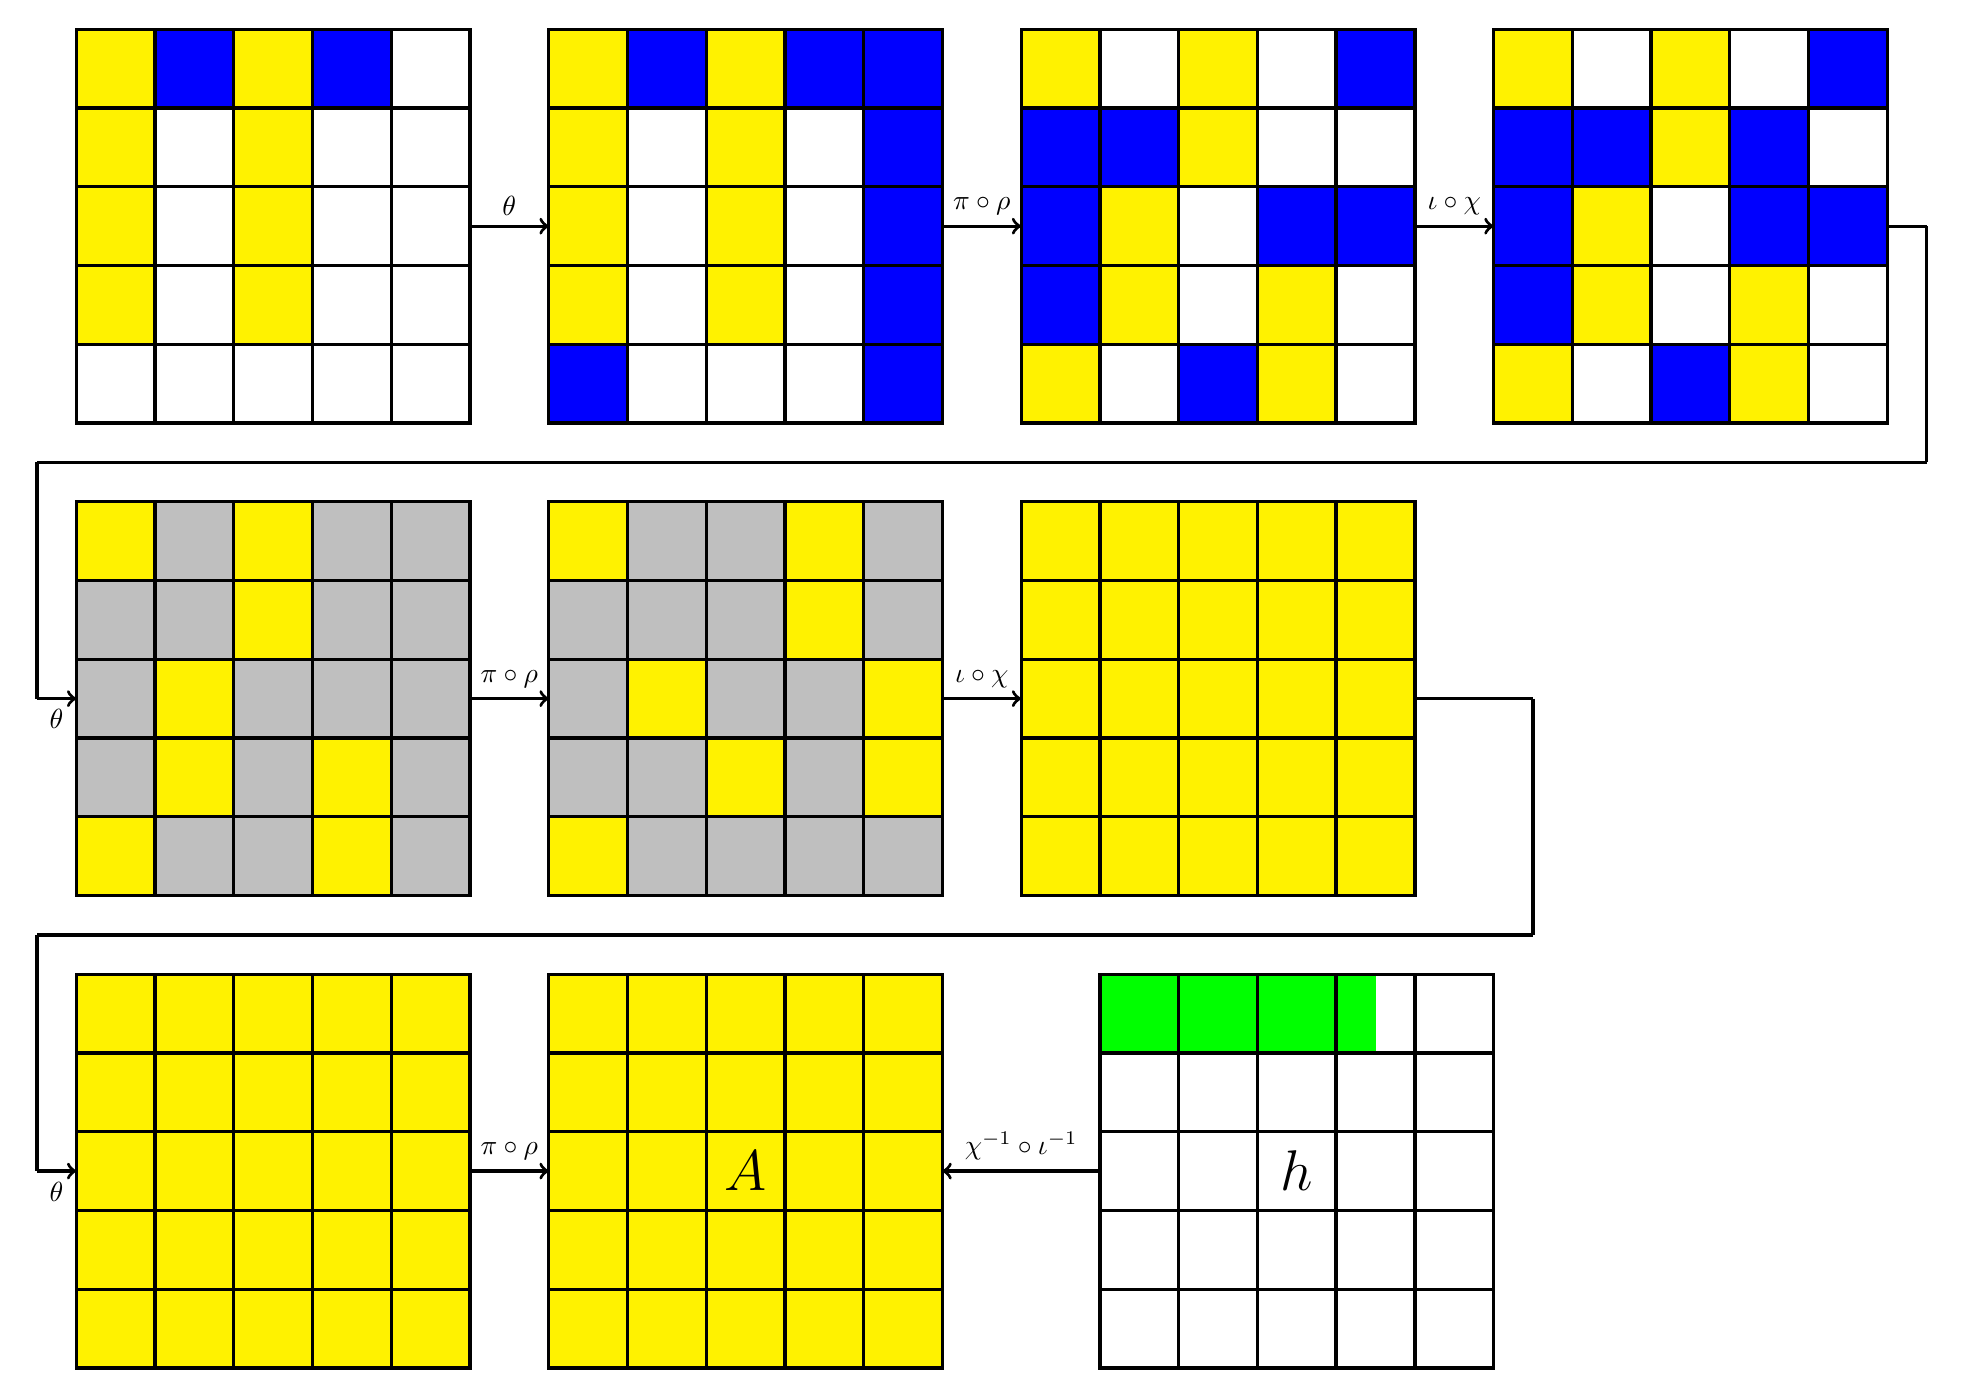
\begin{tikzpicture}
    [%%%%%%%%%%%%%%%%%%%%%%%%%%%%%%
        box/.style={rectangle,draw=black,very thick, minimum size=1cm}
    ]%%%%%%%%%%%%%%%%%%%%%%%%%%%%%%
\definecolor{darkgreen}{rgb}{0.0, 0.7, 0.5}
\foreach \x in {0,1,...,4}{
    \foreach \y in {0,1,...,4}
        \node[box] at (\x,\y){};
}


\foreach \y in {1,2,3,4}
   \node[box,fill=yellow ] at (0,\y){};

\foreach \y in {1,2,3,4}
   \node[box,fill=yellow ] at (2,\y){};

\node[box,fill=blue] at (3,4){};
\node[box,fill=blue] at (1,4){};

\foreach \x in {6,7,...,10}{
    \foreach \y in {0,1,...,4}
        \node[box] at (\x,\y){};
}

\draw [->,very thick] (4.5,2) -- node [above] {$\theta$} (5.5,2);

\foreach \y in {1,2,3,4}
   \node[box,fill=yellow ] at (6,\y){};

\foreach \y in {1,2,3,4}
   \node[box,fill=yellow ] at (8,\y){};

\foreach \y in {0,1,2,3,4}
   \node[box,fill=blue ] at (10,\y){};

\node[box,fill=blue] at (9,4){};
\node[box,fill=blue] at (7,4){};

\node[box,fill=blue] at (6,0){};

\foreach \x in {12,...,16}{
    \foreach \y in {0,1,...,4}
        \node[box] at (\x,\y){};
}

\node[box,fill=yellow] at (15,1){};
\node[box,fill=blue] at (12,1){};
\node[box,fill=blue] at (12,2){};
\node[box,fill=blue] at (12,3){};

\node[box,fill=blue] at (16,4){};
\node[box,fill=blue] at (16,2){};
\node[box,fill=blue] at (15,2){};
\node[box,fill=blue] at (14,0){};
\node[box,fill=blue] at (13,3){};

\draw [->,very thick] (10.5,2) -- node [above] {$\pi \circ \rho$} (11.5,2);

\node[box,fill=yellow ] at (12,4){};
\node[box,fill=yellow ] at (12,0){};

\node[box,fill=yellow ] at (13,1){};
\node[box,fill=yellow ] at (13,2){};

\node[box,fill=yellow ] at (14,3){};
\node[box,fill=yellow ] at (15,0){};
\node[box,fill=yellow ] at (14,4){};

\foreach \x in {18,...,22}{
    \foreach \y in {0,1,...,4}
        \node[box] at (\x,\y){};
}

\node[box,fill=yellow ] at (18,4){};
\node[box,fill=blue ] at (18,3){};
\node[box,fill=blue ] at (18,2){};
\node[box,fill=blue ] at (18,1){};
\node[box,fill=yellow ] at (18,0){};

\node[box,fill=blue ] at (19,3){};
\node[box,fill=yellow ] at (19,2){};
\node[box,fill=yellow ] at (19,1){};

\node[box,fill=yellow ] at (20,4){};
\node[box,fill=yellow ] at (20,3){};
\node[box,fill=blue ] at (20,0){};

\node[box,fill=blue ] at (21,3){};
\node[box,fill=blue ] at (21,2){};
\node[box,fill=yellow ] at (21,1){};
\node[box,fill=yellow ] at (21,0){};

\node[box,fill=blue ] at (22,4){};
\node[box,fill=blue ] at (22,2){};

\draw [->,very thick] (16.5,2) -- node [above] {$\iota \circ \chi$} (17.5,2);

\foreach \x in {0,1,...,4}{
    \foreach \y in {-2,...,-6}
        \node[box,fill=lightgray] at (\x,\y){};
}

\node[box,fill=yellow ] at (0,-2){};
% \node[box,fill=blue ] at (0,-3){};
% \node[box,fill=blue ] at (0,-4){};
% \node[box,fill=blue ] at (0,-5){};
\node[box,fill=yellow ] at (0,-6){};

% \node[box,fill=blue ] at (1,-3){};
\node[box,fill=yellow ] at (1,-4){};
\node[box,fill=yellow ] at (1,-5){};

\node[box,fill=yellow ] at (2,-2){};
\node[box,fill=yellow ] at (2,-3){};
% \node[box,fill=blue ] at (2,-6){};

% \node[box,fill=blue ] at (3,-3){};
% \node[box,fill=blue ] at (3,-4){};
\node[box,fill=yellow ] at (3,-5){};
\node[box,fill=yellow ] at (3,-6){};

% \node[box,fill=blue ] at (4,-2){};
% \node[box,fill=blue ] at (4,-4){};

\draw [-,very thick] (22.5,2) -- node [above] {} (23,2);

\draw [-,very thick] (23,2) -- node [above] {} (23,-1);

\draw [-,very thick] (23,-1) -- node [above] {} (-1,-1);

\draw [-,very thick] (-1,-1) -- node [above] {} (-1,-4);

\draw [->,very thick] (-1,-4) -- node [below] {$\theta$} (-0.5,-4);

\foreach \x in {6,7,...,10}{
    \foreach \y in {-2,...,-6}
        \node[box] at (\x,\y){};
}

\foreach \x in {6,7,...,10}{
\foreach \y in {-2,...,-6}
        \node[box,fill=lightgray] at (\x,\y){};
}

\node[box,fill=yellow ] at (6,-2){};
\node[box,fill=yellow ] at (6,-6){};
\node[box,fill=yellow ] at (7,-4){};
\node[box,fill=yellow ] at (8,-5){};
\node[box,fill=yellow ] at (9,-2){};
\node[box,fill=yellow ] at (9,-3){};
\node[box,fill=yellow ] at (10,-4){};
\node[box,fill=yellow ] at (10,-5){};

\draw [->,very thick]  (4.5,-4) -> node [above] {$\pi \circ \rho$} (5.5,-4) ;

\foreach \x in {12,13,...,16}{
    \foreach \y in {-2,...,-6}
        \node[box] at (\x,\y){};
}

\foreach \x in {12,13,...,16}{
\foreach \y in {-2,...,-6}
        \node[box,fill=yellow] at (\x,\y){};
}

\draw [->,very thick]  (10.5,-4) -- node [above] {$\iota \circ \chi$} (11.5,-4) ;

% 3rd round

\foreach \x in {0,1,...,4}{
    \foreach \y in {-8,...,-12}
        \node[box,fill=yellow] at (\x,\y){};
}

\draw [-,very thick] (16.5,-4) -- node [above] {} (18,-4);

\draw [-,very thick] (18,-4) -- node [above] {} (18,-7);

\draw [-,very thick] (18,-7) -- node [above] {} (-1,-7);

\draw [-,very thick] (-1,-7) -- node [above] {} (-1,-10);

\draw [->,very thick] (-1,-10) -- node [below] {$\theta$} (-0.5,-10);

\foreach \x in {6,7,...,10}{
    \foreach \y in {-8,...,-12}
        \node[box,fill=yellow] at (\x,\y){};
}

\draw [->,very thick]  (4.5,-10) -> node [above] {$\pi \circ \rho$} (5.5,-10) ;

\foreach \x in {13,...,17}{
    \foreach \y in {-8,...,-12}
        \node[box] at (\x,\y){};
}

\draw [<-,very thick]  (10.5,-10) -- node [above] {$\chi^{-1} \circ \iota^{-1}$} (12.5,-10) ;

\foreach \x in {13,...,15}{
    \node[box,fill=green ] at (\x,-8){};
}

\draw[color=green,fill=green] (15.53,-7.53) rectangle (16, -8.47);

\node at (8,-10){\huge $A$};

\node at (15,-10){\huge $h$};


\end{tikzpicture}
\end{document}